\chapter{Design-ul aplicației client}
\section{Introducere}
\par \textbf{În acest capitol, în secțiunea 6.2, se stabilesc funcțiile aplicației client. În secțiunea 6.3 se prezintă conceptul aplicației software și se enumeră tehnologiile folosite la realizarea acestuia în structura următoare: }

\begin{itemize}
\item 6.3.1 - Cercetare a modului de livrare a conținutului educativ în mediul 3D.
\item 6.3.2 - Tehnologii utilizate pentru redarea 3D a lumii virtuale.
\item 6.3.3 - Tehnologii utilizate pentru relizarea interfaței grafice (GUI).
\item 6.3.4 - Tehnologia utilizată pentru comunicarea cu serverul.
\end{itemize}

\par \textbf{ În secțiunea 6.4 se explică mecanismul adoptat pentru atingerea unui scop important, ”scalabilitatea aplicației” . În secțiunea 6.5 se explică mecanismul CERERE-PROCESARE-RASPUNS. În aceeași secțiune se prezintă formatul de reprezentare a datelor transmise între aplicația client și aplicația server. Secțiunea 6.6 este dedicată prezentării diagramei claselor. În secțiunea 6.7 se enunță parametrii testării aplicației client. Rezultatele acestei testări expuse în același capitol. } 

\newpage

\section{Funcțiile aplicației client.}

\par Aplicația client are scop demonstrativ. Implementarea se va executa în cel mai simplu mod posibil, cu interfețe utilizator minimale. Funcțiile de bază ale aplicației client sunt enumerate dar implementarea nu se execută în integralitate.

\textbf{Funcții de bază:}
\begin{itemize}
\item Redarea 3D a obiectelor lumii virtuale.
\item Schimbul de date între aplicație și server, după modelul CERERE - RĂSPUNS.
\item Facilitarea comunicării directe între participanții la procesul de învățare în mediul virtual.
\item Reprezentarea utilizatorilor în mediul virtual prin intermediul avatarelor. Fiecare utilizator va fi reprezentat de un avatar identificabil de către ceilați utilizatori.
\item Facilitarea cooperării între utilizatori.
\item Aplicația, în anumite instanțe, va asista utilizatorul în procesul de învățare. 
\end{itemize}

\section{Conceptul aplicației și tehnologiile utilizate.}

\par Interfața aplicției cu utilizatorul este esențială pentru asugurarea unei experințe cât mai plăcute în timpul utilizării. Pentru realizarea interfețelor se vor respecta următoarele aspecte: simplitate, etichete și denumiri sugestive.
\par Designul interfeței grafice 2D este minimal. Se va dezvolta în principal componenta de redarea 3D a obiectelor din mediul virtual.

\begin{figure}[ht]
    \centering
    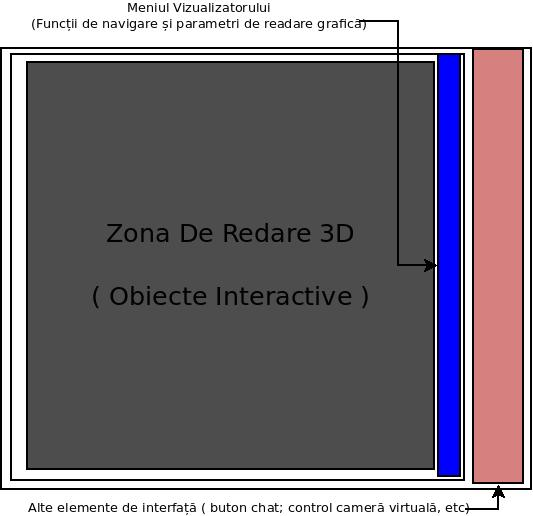
\includegraphics[scale=0.32]{concept}
    \caption{Dispunerea elementelor în interfața grafică}
    \label{fig:vorldd}
\end{figure}

\newpage
\subsection{Modul de livrare a conținutului educativ în mediul 3D}

\begin{figure}[ht]
    \centering
    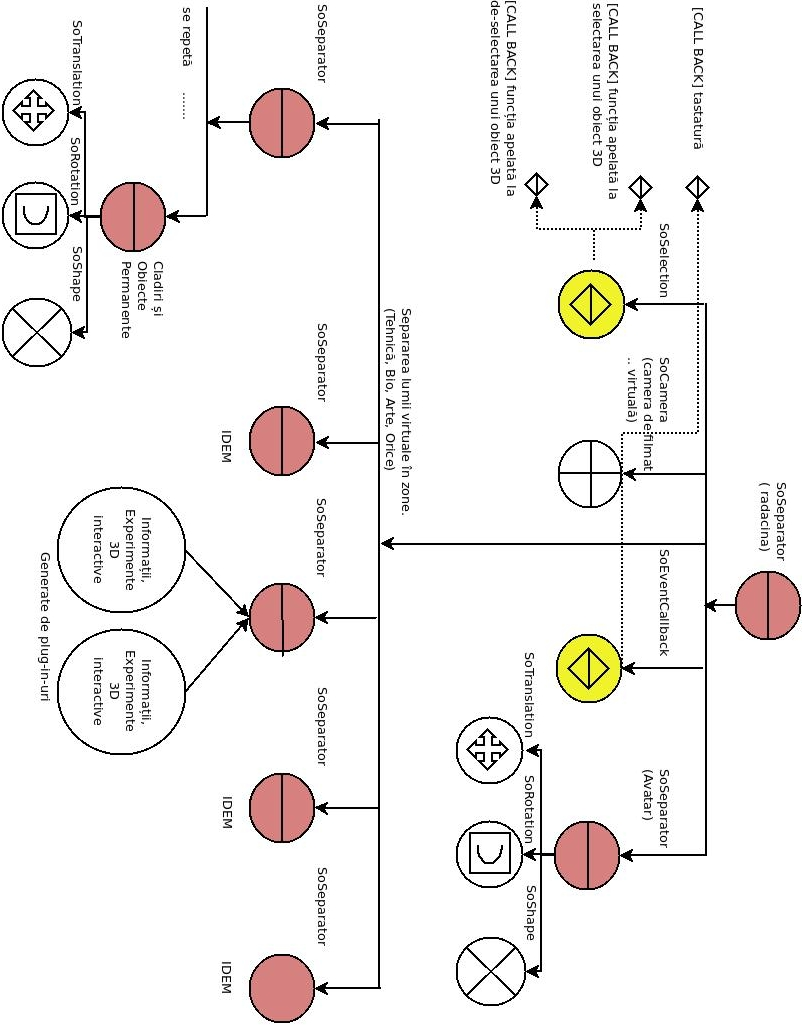
\includegraphics[scale=0.4]{WRLD}
    \caption{Mediul 3D și materialul educativ interactiv}
    \label{fig:vorldd}
\end{figure}

\newpage

\subsection{Tehnologii utilizate pentru redarea 3D a mediului de învățare.}
\subsubsection{Sistemul de operare}
\par Sistemul de operare ales pentru dezvoltarea aplicatiei este GNU/Linux (sitemul de operare GNU + kernelul Linux), distribuția Ubuntu, un sistem de operare modern, foarte asemanător sistemului de operare Unix, dezvoltat de către comunitățile “Free Foftware” și “Open Source”.
\par Motivele alegerii acestui sistem de operare sunt urmatoarele: 
\begin{itemize}
\item Stabilitatea sistemului de operare. 
\item Performanța sistemului de operare. 
\item Simplitatea în instalare și menținere.  
\item Multitasking și managementul memoriei foarte eficient implementate.
\item Compilatoarele, librariile grafice și cele mai importante instrumente pentru dezvoltarea de medii 3D sunt ușor de instalat șconfigurat, sunt gratuite și bine documentate pentru GNU/Linux.
\end{itemize}

\subsubsection{Limbajul de programare}

\par Limbajul de programare ales pentru realizarea aplicației client este C++. Sunt motivat în alegerea mea de urmatoarele caracteristici ale acestui limbaj:  
\begin{itemize}
\item Aplicațiile programate în C++ ruleaza vizibil mai rapid decat aplicațiile realizate în alte limbaje de programare.
\item O multitudine de biblioteci software utile sunt implementate în C++.
\item Aplicația finală poate fi compilată pentru mai multe platforme.
\item C++ este limbajul de programare preferat de dezvoltatorii aplicatii bazate pe grafica 3D.
\end{itemize}
     
\par Compilatorul ales este g++ din colectia GCC (Gnu Compilers Collection). 

\subsubsection{Limbje și biblioteci software utilizate \\ pentru reprezentarea mediului virtual 3D}

\par Când se alege o bibliotecă 3D, factorii care trebuiesc luaţi în considerare sunt: performanța,
existența şi calitatea documentaţiei, platformele care acceptă biblioteca grafică 3D, existenţa unui
format standardizat pentru a descrie obiectele grafice şi interacţiunile obiect, licenţiere etc. Ţinând cont de criteriile menţionate mai sus s-a ales biblioteca Coin3D cu suport VRML (Virtual Reality Modeling
Language). 

\subsubsection{Coin 3D (Open Inventor reimplementat cu suport pentru V.R.M.L.)}
\par \textbf{Generalități}
\par Coin se bazează pe librăria grafică 3D OpenGL (The Open Graphics Library), și își are rădăcinile în Open Inventor 2.1 API, cu care Coin este încă compatibil. Precursorul bibliotecii Coin3D, Open Inventor, își bazează modul de păstrare și manipularea a obiectelor grafice, pe libraria și structura claselor C++ original proiectată pentru SGI.\cite{C04}
\par Open Inventor a devenit repede după lansare biblioteca grafică standard de facto pentru vizualizare 3D și software de simulare vizuală în comunitatea științifică și inginerească, și mai târziu, bază pentru formatul standard VRML1. 
\par Există multe publicații pe subiectul Open Inventor, cele mai importante fiind: “The Inventor Mentor”, “The Inventor Toolmaker”, amandouă fiind recomandate pentru cei ce doresc să învețe sa utilizeze Open Inventor. Aceleași materiale de studiu se pot folosi pentru inițierea în utilizarea librariei grafice Coin3D.\cite{C04}
\par Coin3D a fost dezvoltată independent, de la zero înainte ca Open Inventor să devină open source. Coin și-a atins țelul compatibilității cu standardul Open Invetor 2.1 în toamna anului 2000 și de atunci a fost și-a dezvoltat foarte mult numarul de caracteristici, variind de la suportul pentru sunetul 3D (deficitar pentru sistemul de operare GNU/Linux) la suportul GLSL shader, formate de fișiere suplimentare cum ar fi VRML97, și un numar larg de schimbări interne pentru a ține pasul cu noul OpenGL, optimizat cu o varietate mare de tehnici ce nu erau disponibile la început.\cite{C04} 
\par \textbf{Istoric}
\par Coin își are începuturile în anul 1995, fiind conceput ca o librarie de redare grafică pentru standardul VRML 1.0 . Initial a fost dezvoltată plecând de la librăria Qv a SGI care are rolul de a analiza fisierele în format VRML 1.0. După ani de extindere anevoioasă a bibliotecii soft, începând cu noi funcționalități de redare și exportare precum VRML 1 și VRML 2, în anul 1997 s-a ajuns la o reală nevoie de reproiectatare.\cite{C04}
\par La prima vedere API-ul are o asemănare izbitoare cu Open Inventor. Conceptele utilizate de către Open Inventor sunt deseori amintite ca o bună metodologie de proiectare în multe cărti de inginerie software, astfel că o parte dintre programatorii care s-au ocupat de dezvoltarea acestuia și care aveau deja experiența cu această librarie, au luat conceptul Open Inventor ca un exemplu demn de urmat. Concomitent cu identificarea strategiei de rescriere a codului, s-a luat decizia de colaborare cu membrii comunității Free Software care au contribuit cu o serie de idei tehnice interesante. Ca o urmare firească a acestei colaborări, libraria s-a dezvoltat ca o alternativă liberă la varianta Open Inventor, cu suport pentru sistemele de operare GNU/Linux, IRIX, Windows, Cygwin și Mac OS X.\cite{C04}

\subsubsection{V.R.M.L. (Virtual Reality Modeling Language)}
\par VRML este un limbaj de modelare a lumilor virtuale și un standard internațional pentru descrierea formelor și a scenelor pentru World Wide Web. Organizația responsabilă cu dezvoltarea și publicarea standardului VRML este ”Web 3D Consortium” anterior cunoscută sun numele ”VRML Consortium”. În prezent standardul a ajuns la versiunea a doua.
\par În principiu, o lume virtuală descrisă cu limbajul VRML se poate reprezenta printr-o structură arborescentă în care „nodurile și frunzele” arborelui sunt noduri VRML. 

\begin{figure}[h]
    \centering
    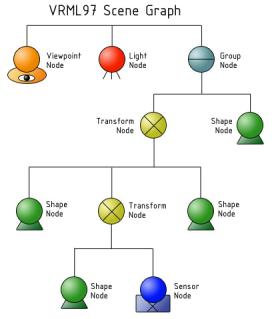
\includegraphics[scale=1.1]{vrml-scene-graph}
    \caption{Graf VRML (exemplu)}
    \label{fig:graphvrml}
\end{figure}

\par Modul în care lumea virtuală este afișată pe display-ul computerului  este influențat de ordinea și amplasarea nodurilor în arbore. Fiecare nod este redat în mod grafic după următoarele reguli:

\begin{itemize}
\item Redarea unui grup de noduri se face în ordine, de regulă, de la stânga la dreapta. Aplicând această regulă la ilustrația precedentă \ref{fig:graphvrml}, putem trage concluzia că nodurile de tip ”transformări” (transform) au efect asupra nodului ”Formă geometrică” (Shape Node) doar dacă sunt amplasate înaintea acestuia.
\item Fiecare nod execută propria afișare și afectează starea următoarelor noduri prin modificarea proprietăților membre. Spre exemplu, un obiect al carui suprafață este reflexivă sau radiantă din puntul de vedere al luminozității, poate afecta modul în care urmatoarele noduri sunt iluminate.
\item Nodurile de tip ”transformare” (Transform Node) se influențează prin combinare (ex: două rotații de 90$^{\circ}$ se acumulează formând o rotație de 180$^{\circ}$ ).
\item Nodurile de tip ”formă geometrică” sunt afișate în modul dictat de starea actuală (ultima culoare setată, ultima luminozitate setată).
\item Nodurile de tip SoSeparator (separatoare), spre diferență de SoGroup (grup), salvează starea actuală înainte de a-i parcurge și afișa nodurile membre. Această stare este restaurată după parcurgerea separatorului. Astfel, nodurile din separator nu afectează nodurile următoare, fiind izolate.
\item Nodurile sunt ”construite” la punctul de coordonate XYZ = (0,0,0) dacă nu sunt afectate de nici o transformare.
\item Sistemul de coordonate VRML este următorul : pentru valori pozitive, axa Y este orientată în sus, axa X este orientată spre dreapta și axa Z este perpendiculară pe axele XY și este orientată spre observator. \ref{fig:vrmlaxes}
\item Pentru efectuarea rotațiilor se aplică regula mâinii drepte. Sensul pozitiv al rotației este sensul invers acelor de ceasornic. Rotația se exprimă în grade radian. \ref{fig:vrmlrot}
\end{itemize} 

\begin{figure}[h]
    \centering
    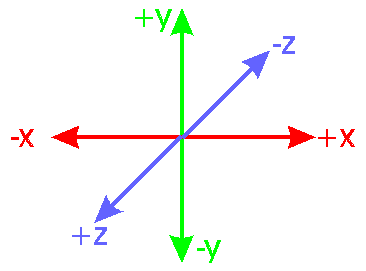
\includegraphics[scale=0.5]{vrmlaxis}
    \caption{Axe}
    \label{fig:vrmlaxes}
\end{figure}

\begin{figure}[h]
    \centering
    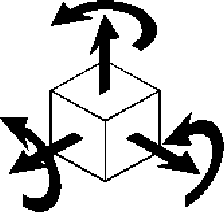
\includegraphics[scale=0.5]{rotation-rule}
    \caption{Rotație}
    \label{fig:vrmlrot}
\end{figure}

\par \textbf{Animații descrise în VRML}
\par Scenele 3D descrise cu ajutorul limbajului VRML pot fi animate și pot fi programate să răspundă la comenzile utilizatorului. Acestă interacțiune se poate realiza în două moduri: programatic, prin accesarea și modificarea nodurilor grafului scenei VRML prin rutinele unui program dezvoltat de utilizator (în C++/Python/etc); sau prin folosirea mecanismulor de descriere a interacțiunilor și animațiilor pus la dispoziție de limbajul VRML.
\par Interactivitatea în VRML se realizează prin transmiterea de valori ale ”proprietăților” între diversele noduri ale grafului VRML. Când un nod trimite informații către un alt nod, se crează un \textbf{eveniment (”event”)}, o structură ce transportă două informații date (valori) și informație referitoare le timp (timestamp) pentru exprimarea momentului în care evenimentul s-a produs, cu scopul asigurării integrității logice pentru secvențele de evenimente [CITE COMENT Rohel]. Mecanismul animației presupune crearea unei conexiuni explicite între noduri cu ajutorul construcției sintactice \textbf{ROUTE} între ”câmpurile” ce stochează atributele nodurilor implicate în animație. Majoritatea nodurilor sunt construite după structura:
\begin{verbatim}
nod { 
   camp             (field)         ; inaccesibil
   eveniment primit (eventIn)       ; permite doar scriere
   eveniment emis   (eventOut)      ; permitere doar citire
   câmp expus       (exposedField)  ; permite citire și srcirere
}
\end{verbatim} 
Evenimentele transmise prin câmpul eventOut al unui nod, vor putea fi recepționate de un al doilea nod prin câmpul eventIn, având ca efect animația nodului receptor.	\ref{fig:vrmlanim}	

\begin{figure}[h]
    \centering
    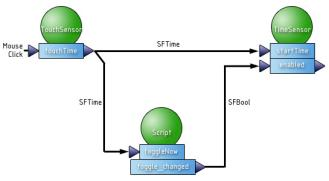
\includegraphics[scale=1.5]{vrml-anim}
    \caption{ANIMAȚIE VRML}
    \label{fig:vrmlanim}
\end{figure}
% Roehl, B., et al. (1997), Late Night VRML 2.0 with Java. Emeryville: Ziff-Davis.
\newpage
\par Exemplu: (Orientarea obiectului grafic se modifică în timp, din momentul activării senzorului de atingere)
\begin{verbatim}
# VRML V2.0 utf8 

DEF Touch TouchSensor { } 
DEF Timer1 TimeSensor { } 
DEF Rot1 OrientationInterpolator { } 

DEF Frame1 Transform { 
	children [ 
		Box { }   
		] 
} 

ROUTE Touch.touchTime TO Timer1.set_startTime 
ROUTE Timer1.fraction_changed TO Rot1.set_fraction 
ROUTE Rot1.value_changed TO Frame1.set_rotation

\end{verbatim}

\subsection{Tehnologii utilizate pentru relizarea interfaței grafice (GUI)}
\par Interfețele grafice se vor implemeta folosind atât bibilotecile software Qt/SoQt cât și tehnologii Web/HTML. Interfețele Web sunt adoptate deoarece implementarea lor necesită mai puțin timp și sunt mult mai dinamice decât interfețele implemetate în c++ utilizând bibliotecile Qt/SoQt.

\subsubsection{Qt}

\par Qt este un cadru software pentru programarea aplicațiilor multi-platformă și pentru dezvoltarea de interfețe grafice folosind  ca limbaje: C++, QML, CSS și JavaScript. Librariile Qt și uneletele de dezvoltare sunt eliberate prin licențe compatibile cu modelul ”open source”. 
\par Qt implementează metode inteligente pentru realizarea comunicării între divesrele obiecte ale interfeței grafice. Metoda constă în conectarea evenimentelor prelute de elementele de interfță la rutinele asociate cu aceste evenimente sau conectarea la alte evenimente. Acest lucru se realizează automat, cu ajutorul unui meta-compilator care generează codul necesar conectarii evenimentelor (SIGNAL) la rutine (SLOT). \ref{fig:sig-slot}

\begin{figure}[h]
    \centering
    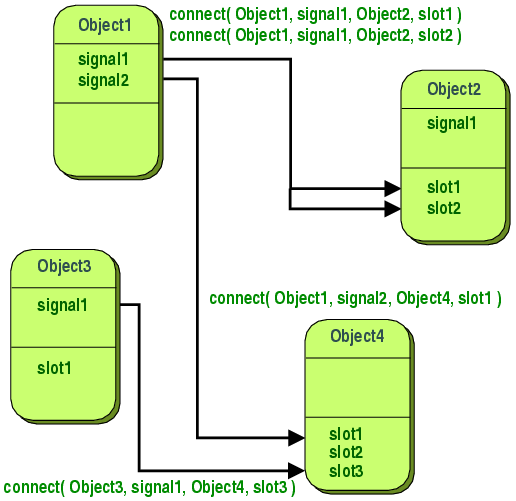
\includegraphics[scale=0.5]{qtconn}
    \caption{Mecanismul SIGNAL-SLOT}
    \label{fig:sig-slot}
\end{figure}

\newpage
\subsubsection{SoQt}
\par SoQt furnizează programatorului o interfață de nivel înalt în C++. Librăria, include o ierarhie de clase cu rol de componentă de vizualizare (viewers), cu funcționalități diferite, împreună cu o serie de modalități de control a interacțiunii dintre camerele virtuale de filmat și scena 3D. SoQt este practic liantul dintre librăriile de interfețe Qt și Coin 3D.
\subsubsection{Interfețe Web/HTML prin mecanismul ”QtWebKit Bridge”}
\par Mecanismul ”WebKit bridge” este parte a bibliotecii sotware Qt. Prin acest mecanism se facilitează accesul obiectelor codificate in JavaScript la rutinele codificate în c++ în aplicația realizată cu ajutorul bibliotecii software Qt. În acest fel, o pagină web poate fi programată ca o interfață pentru un program codificat în c++. 
\subsection{Tehnologia utilizată pentru comunicarea cu serverul}

\par Viteza de execuție a aplicațiilor codificate în C++ și existența librariei Coin3D, este motivul alegerii acestui limbaj pentru implementarea aplicației client. Ultimul standard adoptat de ISO include extensii pentru limbaj și adaugarea de module noi la librăria standard. Cea mai binevenită modificare este suportul pentru programarea firelor de execuție în modelul tehnicii OOP. 
\par Pentru programarea rețelelor de calculatoare nu există suport modern, acest aspect fiind în agenda ISO pentru următorul standard. Pentru acest ”task” am folosit librăria Boost Asio, o subcomponentă a biblotecii software Boost. 
\par Boost Asio implemetează un model modern bazat pe modelul OOP, pentru programarea asincronă a operațiilor I/O la nivel scăzut și programarea aplicațiilor pentru rețele de calculatoare (cu asincronism în ce privește trimiterea/primirea de date în rețea). \ref{fig:asio}

\begin{figure}[h]
    \centering
    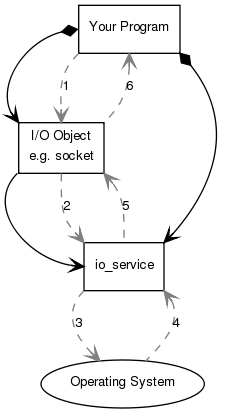
\includegraphics[]{sync_op}
    \caption{Mecanismul I/O asincron}
    \label{fig:asio}
\end{figure}

\section{Decizie privind design-ul aplicației client.}
\par Se va urmări o cît mai mare flexibilizare a sistemului, astfel încât dezvoltarea ulterioară sa fie cât mai facilă. Se are în vedere folosirea mecanismului de extindere dinamică a funcționalității sistemului prin ”plug-in”-uri. 	Plugin-urile vor putea fi descărcate din surse externe în timpul rulării aplicației client, și incluse dinamic în aplicație, fără a se întrerupe rularea programului. Un plug-in va prelua funcția de încărcare de cursuri interactive și activități educative diverse. 

	 Un plug-in respectă următoarea interfață:
\begin{verbatim}
#ifndef L3DCLIENT_PLUGIN_H
#define L3DCLIENT_PLUGIN_H

#include <Inventor/nodes/SoSeparator.h>
#include <string>
 
  //interfața plug-in
  extern "C" void get_plug_in( std::string data, SoSeparator* insertionPoint );
  //pointer la o funcție cu aceeiași parametri și tip returnat ca plug-in-ul
  typedef void (*PLUG_IN)( std::string , SoSeparator*);

#endif
\end{verbatim}	
	
\par Plug-inurie sunt în fapt funcții standardizate, compilate în librării dinamice ”Shared Object”. Descărcarea librăriilor de pe internet se va realiza prin apelarea comenzii Linux wget. 
\par Compilarea bibliotecilor software dinamice se efectuează cu specificarea unor parametri speciali pentru compilator.
\begin{itemize}
\item \textbf{-Wall}, afișează toate mesajele de alarmă
\item \textbf{-fPIC}, ”Position independent code”; pubctul de încărcare a instrucțiunilor variază la bibliotecile dinamice. 
\item \textbf{-c}, doar compilare 
\item \textbf{-Wl,-snoname,<name>}, instrucțiuni către link-editor pentru a genera obiecte dinamice
\end{itemize}
Următorul script crează biblioteci software dinamice ce pot utiliza clase Qt, Boost și Coin:
\begin{verbatim}
#!/bin/bash
# ->  mod de foflosire: 
# $>  build_lib.sh <sursa.cpp> <denumire fisier obiect> <nume biblioteca>
# ->  DOAR sursei .CPP i se adauga extensia !!!!!!!!!!!!!!!!!!!!!!!!!!!!! 

CPPFLAGS_COIN=`soqt-config --cppflags`
CXXFLAGS_COIN=`soqt-config --cxxflags`
LDFLAGS_COIN=`soqt-config --ldflags`
LIBS_COIN=`soqt-config --libs`

CPPFLAGS_QT=`soqt-config --cppflags`
CXXFLAGS_QT=`soqt-config --cxxflags`
LDFLAGS_QT=`soqt-config --ldflags`
LIBS_QT=`soqt-config --libs`
INCLUDEDIR_QT=" -I/usr/include/qt4 -I/usr/include/qt4/QtCore \
                -I/usr/include/qt4/QtGui -I/usr/include/qt4/QtOpenGL \
                -I/usr/include/qt4/QtWebKit "

BOOST_CPPFLAGS=" -pthread " 
BOOST_FILESYSTEM_LDFLAGS=" -L/usr/local/lib -Wl,-R,/usr/local/lib "
BOOST_FILESYSTEM_LIBS=" -lboost_filesystem "
BOOST_SYSTEM_LDFLAGS=" -L/usr/local/lib -Wl,-R,/usr/local/lib "
BOOST_SYSTEM_LIBS=" -lboost_system "
BOOST_THREAD_LDFLAGS=" -L/usr/local/lib -Wl,-R,/usr/local/lib "
BOOST_THREAD_LIBS=" -lboost_thread -lboost_system -pthread "

#
# [ -Wall ] display all warnings
# [ -fPIC ] generate Position Independent Code
#
#  MODEL g++ -c -Wall -fPIC plugin1.cpp  -o plugin1.o

g++ -std=c++11 -c -Wall -fPIC $INCLUDEDIR_QT $1 -o $2.o 

#
# [ -Wl,-snoname,<name> ] instuct the linker the
# linker to generate a Dynamic Shared Objects
# instead of an application
#
g++ -std=c++11 $BOOST_CPPFLAGS $CPPFLAGS_COIN $CXXFLAGS_COIN $CPPFLAGS_QT  \
     $CXXFLAGS_QT -I$INCLUDEDIR_QT -shared -Wl,-soname,$3.so -o $3.so $2.o \
     $BOOST_SYSTEM_LDFLAGS $BOOST_SYSTEM_LIBS $BOOST_THREAD_LIBS  \
     $BOOST_THREAD_LDFLAGS $BOOST_FILESYSTEM_LDFLAGS $BOOST_FILESYSTEM_LIBS \
     $LDFLAGS_COIN $LIBS_COIN  $LDFLAGS_QT $LIBS_QT
	
\end{verbatim}
\newpage
\par \textbf{Exemplu de implementare a unui plug-in}
\par Exemplul listat este plug-in-ul care are rolul de a crea si anima avatarele celorlalți utilizatori. Acestea își schimbă orientarea și poziția în spațiu la fiecare 0.5 secunde. Parametrii furnizați de aplicație plug-in-ului reprzintă:

\begin{itemize}
\item Un număr variabil de informații și parametri primiți de la server, în format XML, reprezentînd numele acțiunii ed executat la nivelul aplicației client și datele necesare pentru implemetarea acestei acțiuni.
\item Un pointer spre un ”separator” al lumii virtuale, reprezentând zona în care programatorul plug-in-ului poate insera grafica 3D dorită.
\end{itemize}

\begin{verbatim}
#include "../src/plugin.h"
#include "../src/vrml_utils.h"
#include <Inventor/nodes/SoSeparator.h>
#include <Inventor/nodes/SoTranslation.h>
#include <Inventor/nodes/SoRotation.h>
#include <Inventor/nodes/SoCone.h>
#include <string>
#include <iostream>
#include <cstdlib>
#include <boost/property_tree/ptree.hpp>
#include <boost/property_tree/xml_parser.hpp>
#include <sstream>

#include "../src/vrml_utils.cpp"

extern "C" void get_plug_in( std::string data, SoSeparator* insertionPoint )
{

  using boost::property_tree::ptree;
  ptree pt;

  std::stringstream streammed_msg;
  streammed_msg<<data;

  read_xml(streammed_msg, pt);

  std::string action = pt.get<std::string>("response.action");
  std::string gender = pt.get<std::string>("response.avatar_type_id");
  std::string name = pt.get<std::string>("response.other_user");
 
  std::string rotN = "MOC_ROTATE_"+name;
  std::string movN = "MOC_MOVE_"+name;
 
  //create grapichs first time only
  SoSeparator* _3d_obj = (SoSeparator*)findNode(name.c_str(),insertionPoint);

  std::cout<<std::endl<<data;
  if( _3d_obj == NULL )
    {
      std::cout<<std::endl<<"CREATE A MOC AVATAR";

      SoTranslation *translation = new SoTranslation;
      translation->translation.setValue(0.1,0,0);
      translation->setName( movN.c_str() );
      SoRotation *rotation = new SoRotation;
      rotation->rotation.setValue(SbVec3f(0, 1, 0), 0.1);
      rotation->setName( rotN.c_str() );

      _3d_obj = new SoSeparator;
      _3d_obj->setName(name.c_str());
      _3d_obj->addChild( translation );
      _3d_obj->addChild( rotation );

      if ( gender == "0" )
	  {
	  _3d_obj->addChild(
	      get_scene_graph_from_file("/usr/local/share/l3dclient/avatar_male.wrl")
	      );
	  }
      else
	  {
	  _3d_obj->addChild( 
	      get_scene_graph_from_file("/usr/local/share/l3dclient/avatar_female.wrl")
	      );
	  }

      insertionPoint->addChild( _3d_obj );
    }
  //end create graphics

  //execute code for the current action
  if ( action == "rotate" )
    {
      std::string s_angle = pt.get<std::string>("response.degrees");
      float angle = std::stof( s_angle.c_str() );
      SoRotation* rotation = (SoRotation*) findNode( rotN.c_str(), insertionPoint );
      if ( rotation == NULL )
	{
	  rotation = new SoRotation;
	  rotation->setName( rotN.c_str() );
	  _3d_obj->addChild( rotation );
	}

      rotation->rotation.setValue(SbVec3f(0, 1, 0), angle);
    }
  else if ( action == "move" )
    {
      float x,z;
      
      std::string s_X = pt.get<std::string>("response.x");
      x = std::stof( s_X.c_str() );
      std::string s_Z = pt.get<std::string>("response.z");
      z = std::stof( s_Z.c_str() );
      
      //SbVec3f pos(x,y,z);
      SoTranslation* translation = (SoTranslation*) findNode( movN.c_str(), insertionPoint );
      if ( translation == NULL )
	{

	  translation = new SoTranslation;
	  translation->setName( movN.c_str() );
	  _3d_obj->addChild( translation );
      
	}
      translation->translation.setValue(x,0.0,z);
    
    }
  else if ( action == "talk" )
    {
		// TO DO ... chat action
    }


}

\end{verbatim}

\section{Comnezi către server}

\par Instrucțiunile trimise către server reprezintă șiruri de caractere ce se încadrează în următorul tipar:
 
\begin{verbatim}
        @<COMANDA> <parametrul 1> <parametrul 2> ... <parametrul 2>
\end{verbatim} 
Răspunsul primit de aplicația client este în format XML în una din următoarele forme :

\begin{verbatim}
Excepții / Mesaje de eroare
<?xml version="1.0" encoding="UTF-8"?>"
<response>
   <type></type>
   <exception>
     <message> .... </message>
  </exception>
</response>

Mesaje Valide
<?xml version="1.0" encoding="UTF-8"?>
<response>
  <type></type>
  <name></name>
  <client_plugin></client_plugin>
  <client_plugin_source></client_plugin_source>
  <raw> </raw>
</response>
\end{verbatim}

\par Schimbul de date între client și server formează o buclă completă (CLIENT)-(SERVER)-(CLIENT/CLIENȚI). 
Primul pas este reprezentat de expedierea unei comenzi dinspre client către server, sub forma unui șir de caractere. Primul caracter este ”@” urmat fără spațiu de un nume unic ce are rol de ”selector” de operație la nivelul serverului. Selectorul poate fi urmat de unul sau mai mulți parametri separați prin spații. Comanda expediată, la nivelul serverului este despărțită în elementele constituente: selector de comandă și lista de parametri. Selectorul de comandă este folosit pentru a obține din registrul de comenzi a serverului următoarele informații utile:
\begin{itemize}
\item Numele plug-in-ului ce va prelucra răspunsul serverului la nivelul aplicției client.
\item Adresa web de la care aplicația client poate încărca plug-inul client.
\item Numele plug-in-ului care va procesa la nivelul serverului comanda primită de la aplicația client.
\end{itemize}
Pe baza informațiilor de mai sus, serverul îsi incarcă propriul plug-in de prelucrare a comenzii de la aplicația client (cu parametrii necesari), execută prelucrarea datelor primite de la client și returnează o comanda în format XML cu următoarele informații:

\begin{itemize}
\item tipul comenzii în blocul ”type”
\item numele comenzii în blocul ”name”
\item numele plug-in-ului ce se va executa la nivelul aplicației client, în blocul XML ”client\_plugin”
\item adresa web de la care acest plug-in se poate descărca, în blocul XML ”client\_plugin\_source”
\item parametrii de furnizat plug-in-ului client, în blocul XML ”raw”
\end{itemize}
Această comandă este transmisă aplicației client sau mai multor clienți, în funcție de tipul comanzii. Aplicația client preia mesajul XML și execută în ordine următoarele operații:

\begin{itemize}
\item interpretează comanda XML pentru a extrage numele plug-in-ului asociat acestei comenzi
\item extrage pararmetrii de furnizat plug-in-ului
\item verifică dacă plug-in-ul este deja incărcat in memorie 
\item dacă  plug-in-ul nu este încărcat, se execută încărcarea dinamică a acestuia de la adresa extrasă din comanda XML
\item plug-in-ul se execută cu lista de parametri extrasă din comandă
\end{itemize}

\begin{figure}[h]
    \centering
    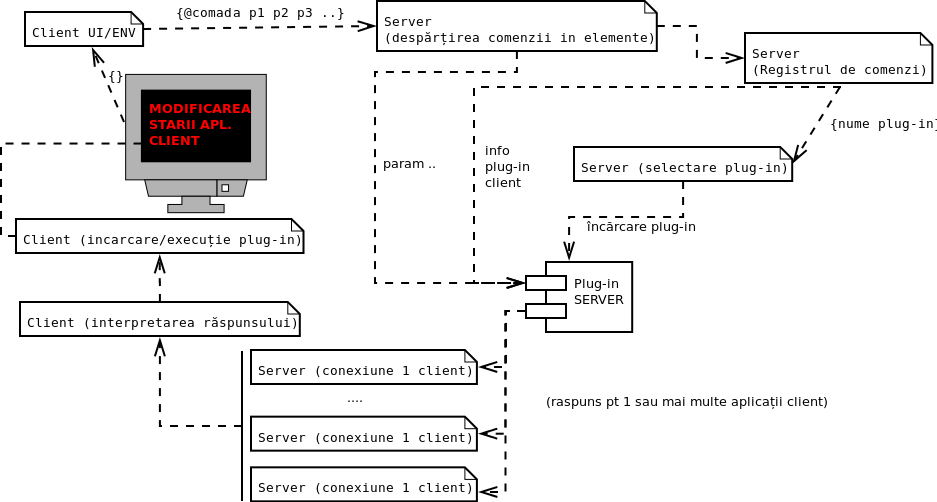
\includegraphics[scale=0.33]{loop}
    \caption{Bucla schimbului de informații între client și server}
    \label{fig:loop}
\end{figure}


\section{Diagrama claselor}
\begin{figure}[h]
    \centering
    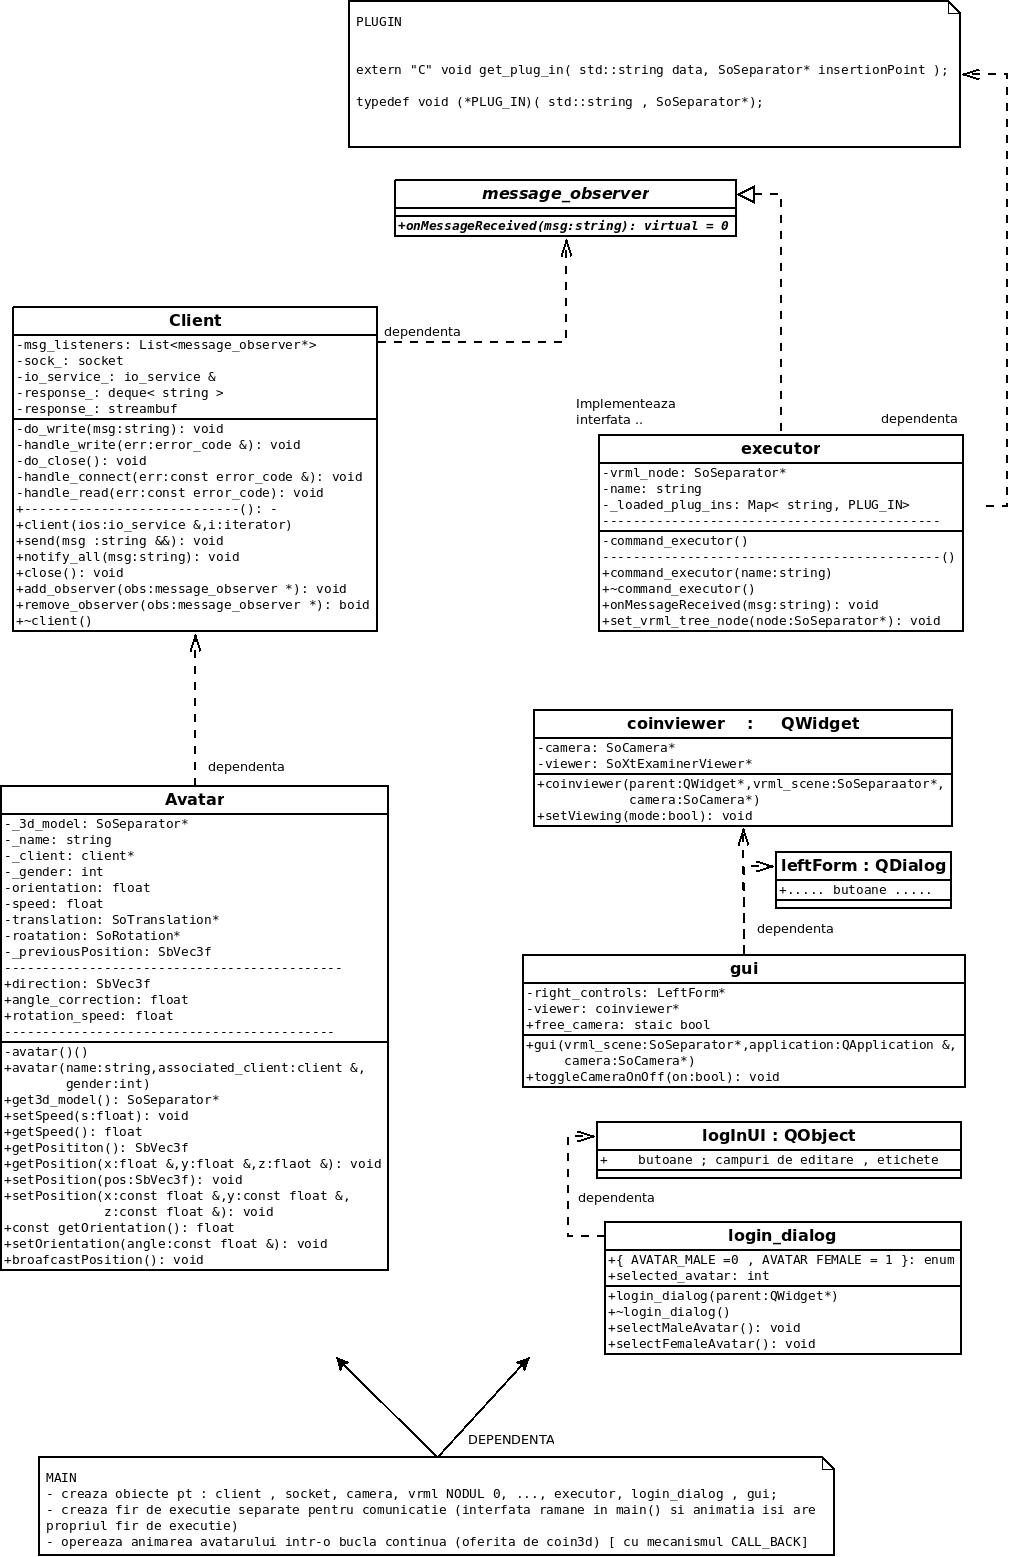
\includegraphics[scale=0.27]{UMLCL}
    \caption{Diagrama claselor aplicației client}
    \label{fig:loop}
\end{figure}

\section{Test}
\par Deoarece o metodă automată pentru testarea întregii aplicații este foarte complexă, se recurge la testarea vizuală, constând în verificarea modului în care perspectiva vizuală dintre două avatare este corectă, și în verificarea modului în care mediul virtual este redat din punct de vedere estetic.
\begin{figure}[ht]
    \centering
    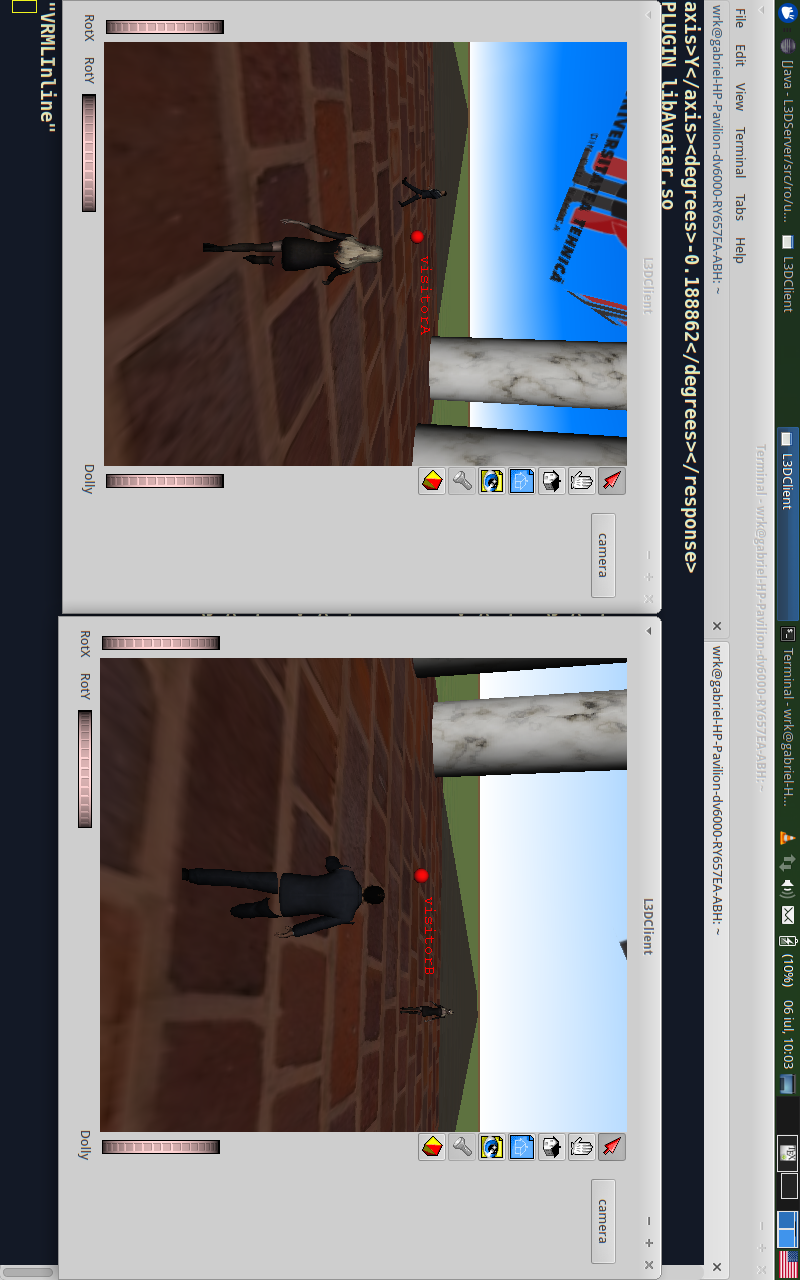
\includegraphics[scale=0.35]{CASTRUM0}
    \caption{Test - avatare - față în față }
    \label{fig:loop}
\end{figure}
\begin{figure}[ht]
    \centering
    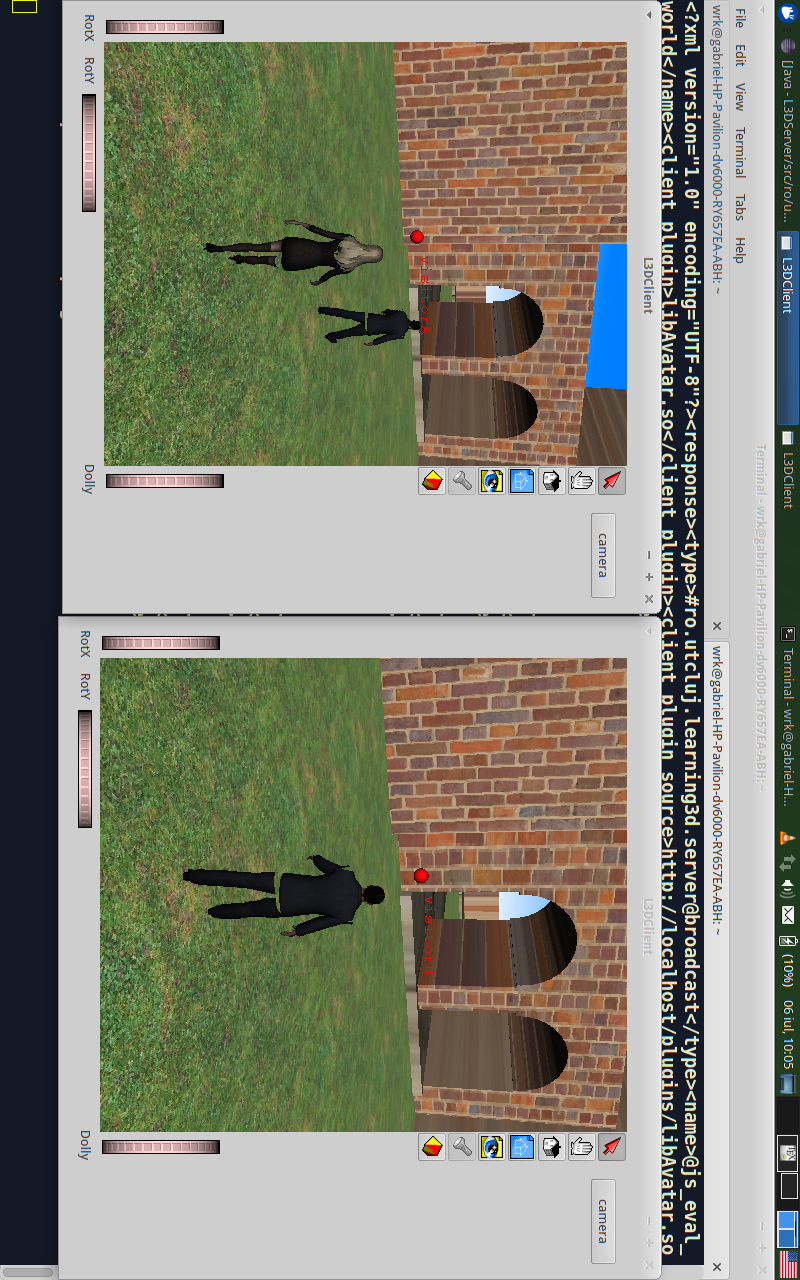
\includegraphics[scale=0.4]{P0}
    \caption{Test - avatare aliniate la intrarea într-o fortificație romană (3D)}
    \label{fig:loop}
\end{figure}